\documentclass{beamer}
\usepackage[utf8]{inputenc}
\usepackage[spanish]{babel}
\usepackage{graphicx}
\usepackage{verbatim}
\usepackage{moreverb}
\usepackage{amsmath}
\usepackage{amsfonts}
\usepackage{amssymb}
\usepackage{fancybox}
\usepackage{float}
\usepackage{fancyvrb}
\usepackage{color}
\usepackage{hyperref}
\usepackage{multirow}
\mode<presentation>
\usepackage{default}

\usetheme{Madrid}

\author{Grupo 5}
\title{Redes de Hopfield}
\subtitle{Trabajo Práctico Especial 3}
\institute[Sistemas de Inteligencia Artificial]{Sistemas de Inteligencia Artificial}

\begin{document}

\maketitle
\begin{frame}
\begin{block}{Introducción}
\begin{itemize}
\item Se nos entregaron 25 patrones a memorizar, todos tenían la misma resolución, aunque algunas imágenes se les tuvo que modificar el formato para que sean compatibles.
\item Se usa redes de Hopfield como memoria direccionable por el contenido.
\end{itemize}

\end{block}
\end{frame}
\begin{frame}{Evaluación y condición de corte}
\begin{block}{Evaluación y condición de corte}
\begin{itemize}
\item Forma asincrónica
\item Luego de 4096 rondas, todas las neuronas han actualizado su estado.
\item Se considera que el patrón de entrada convergió a un estado dado cuando las 4096 rondas arrojan el mismo resultado.
\end{itemize}
\end{block}
\end{frame}

\begin{frame}{Estabilidad de patrones}
\begin{block}{Estabilidad de patrones}
Se calcula el \emph{crosstalk} para cada posición del patrón
\begin{equation}
\mbox{estable}(\xi^\mu) = \left\{ \begin{array}{ll}
\mbox{\textbf{verdadero}} & \forall i \mbox{ crosstalk}(\xi^\mu_i) < 1 \\
\mbox{\textbf{falso}} &\mbox{ en otro caso.}
\end{array} \right.
\end{equation}
\end{block}
\end{frame}

\begin{frame}{Estados espurios y cuencas de atracción}
\begin{block}{Estados espurios y cuencas de atracción}
Se desarrollaron tres \textit{scripts} diferentes, con el fin de generar patrones que puedan caer en cuencas de atracción de estados espurios de la red. \\

\begin{itemize}
\item \textbf{invert:} invierte el patrón que se le indica.
\item \textbf{mixPatterns:} genera todas las posibles combinaciones lineales con coeficientes en 1 de los patrones que se le indican.
\item \textbf{noise:} genera a partir de un patrón de entrada un nuevo patrón aplicándole un ruido de densidad $d$.
 \end{itemize}
 \end{block}
\end{frame}

\begin{frame}{Remoción de estados espurios}
\begin{block}{Remoción de estados espurios}
Se implemente la remoción de estados espurios de la siguiente forma: \\
\begin{enumerate}
 \item Se aplica a todos los pesos, el término corrector de la ecuación \ref{Eq:spu} siendo $S^f$ el estado espurio que se desea eliminar.
 \item Se evalúa el patrón que convergía a ese estado espurio, si este sigue convergiendo se vuelve al paso 1.
\end{enumerate}
\begin{equation}
  \label{Eq:spu}
   \Delta w_{ij} = -\dfrac{\epsilon}{N} S^{f}_{i} S^{f}_{j}
\end{equation}
\end{block}
\end{frame}

\begin{frame}{Pruebas}
\begin{block}{Pruebas}
Para todas las pruebas se utiliza una red que almacena los siguientes patrones, que mediante la regla de \emph{conjuntoEstable} se comprobó que todos los patrones eran estables en esta red.
\begin{figure}[h!]
 \centering
 \fbox{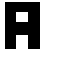
\includegraphics{../../src/img/original/a.png}}
 \fbox{
\includegraphics{../../src/img/original/line2.png}}
 \fbox{
\includegraphics[scale=1.34]{../../src/img/original/windows.png}}
 \caption{Patrones almacenados en la prueba de estabilidad}
 \label{Fig:stability}
\end{figure}
\end{block}
\end{frame}

\begin{frame}{Pruebas: atracción}
\begin{block}{Atracción}
\begin{figure}[h!]
 \centering
 \fbox{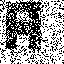
\includegraphics[scale=0.5]{../../src/img/results/a_noise_50.png}}
 \fbox{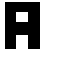
\includegraphics[scale=0.5]{../../src/img/original/a.png}}
 
 \fbox{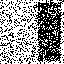
\includegraphics[scale=0.5]{../../src/img/results/line_noise_50.png}}
 \fbox{
\includegraphics[scale=0.5]{../../src/img/original/line2.png}}
 
 \fbox{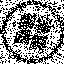
\includegraphics[scale=0.5]{../../src/img/results/win_noise_50.png}}
 \fbox{
\includegraphics[scale=0.67]{../../src/img/original/windows.png}}
 \caption{Ruido de densidad del 50\%.}
 \label{Fig:noise50}
\end{figure}
\end{block}
\end{frame}

\begin{frame}{Pruebas: atracción}
\begin{block}{Atracción}
\begin{figure}[h!]
 \centering
 \fbox{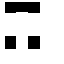
\includegraphics[scale=0.5]{../../src/img/tests/a_incomplete1.png}}
 \fbox{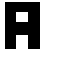
\includegraphics[scale=0.5]{../../src/img/original/a.png}}
 
 \fbox{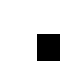
\includegraphics[scale=0.5]{../../src/img/tests/line2_incomplete1.png}}
  \fbox{
\includegraphics[scale=0.5]{../../src/img/original/line2.png}}
 
 \fbox{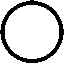
\includegraphics[scale=0.67]{../../src/img/tests/win_incomplete1.png}}
\fbox{
\includegraphics[scale=0.67]{../../src/img/original/windows.png}}
 \caption{Versiones incompletas de los patrones almacenados.}
 \label{Fig:incomplete1}
\end{figure}
\end{block}
\end{frame}

\begin{frame}{Pruebas: atracción}
\begin{block}{Atracción}
\begin{figure}[h!]
 \centering
 \fbox{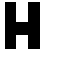
\includegraphics[scale=0.5]{../../src/img/original/h.png}}
 \fbox{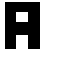
\includegraphics[scale=0.5]{../../src/img/original/a.png}}
 
  \fbox{
\includegraphics[scale=0.5]{../../src/img/original/line1.png}}
 \fbox{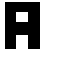
\includegraphics[scale=0.5]{../../src/img/original/a.png}}
 
 \fbox{
\includegraphics[scale=0.67]{../../src/img/original/mac.png}}
 \fbox{
\includegraphics[scale=0.5]{../../src/img/results/result_mac_windows.png}}
 \caption{Patrones que no fueron almacenados en la red.}
 \label{Fig:others}
\end{figure}
\end{block}
\end{frame}

\begin{frame}{Pruebas: patrones inversos}
\begin{block}{Patrones inversos}
\begin{figure}[h!]
 \centering
 \fbox{
\includegraphics[scale=0.5]{../../src/img/results/a_inv.png}}
 \fbox{
\includegraphics[scale=0.5]{../../src/img/results/a_inv.png}}
 
  \fbox{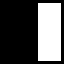
\includegraphics[scale=0.5]{../../src/img/results/line_inv.png}}
 \fbox{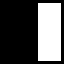
\includegraphics[scale=0.5]{../../src/img/results/line_inv.png}}
 
 \fbox{
\includegraphics[scale=0.5]{../../src/img/results/win_inv.png}}
 \fbox{
\includegraphics[scale=0.5]{../../src/img/results/win_inv.png}}
 \caption{Patrones inversos como entrada.}
 \label{Fig:inverts}
\end{figure}
\end{block}
\end{frame}

\begin{frame}{Pruebas: combinación de patrones almacenados}
\begin{block}{Combinación de patrones almacenados}
\begin{figure}[h!]
 \centering
 \fbox{
\includegraphics[scale=0.5]{../../src/img/results/mix1.png}}
 \fbox{
\includegraphics[scale=0.5]{../../src/img/results/mix1.png}}
 
  \fbox{
\includegraphics[scale=0.5]{../../src/img/results/mix2.png}}
 \fbox{
\includegraphics[scale=0.5]{../../src/img/results/mix2.png}}
 \caption{Combinaciones lineales de los patrones almacenados como entrada}
 \label{Fig:mix}
\end{figure}
\end{block}
\end{frame}

\begin{frame}{Pruebas: remoción de patrones espurios}
%\begin{block}{Remoción de patrones espurios}
\begin{figure}[h!]
 \centering
 \fbox{
\includegraphics[scale=0.5]{../../src/img/results/a_inv.png}}
 \fbox{
\includegraphics[scale=0.5]{../../src/img/results/rem_spu_1.png}}
 
 \fbox{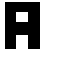
\includegraphics[scale=0.5]{../../src/img/original/a.png}}
 \fbox{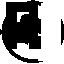
\includegraphics[scale=0.5]{../../src/img/results/rem_spu_2.png}}
 \caption{Removiendo el estado inverso del patrón a.png}  
 \label{Fig:spu1}
\end{figure}

\begin{figure}[h!]
 \centering
 \fbox{
\includegraphics[scale=0.5]{../../src/img/results/mix1.png}}
 \fbox{
\includegraphics[scale=0.5]{../../src/img/results/rem_spu_3.png}}
 
  \fbox{
\includegraphics[scale=0.5]{../../src/img/results/mix2.png}}
 \fbox{
\includegraphics[scale=0.5]{../../src/img/results/rem_spu_4.png}}
 \caption{Removiendo el patrón de la mezcla de los patrones almacenados.} 
 \label{Fig:spu2}
\end{figure}
%\end{block}}
\end{frame}

\begin{frame}{Prueba de energía}
\begin{block}{Prueba de energía}
\begin{figure}[h!]
 \centering
 \fbox{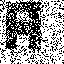
\includegraphics[scale=0.5]{../../src/img/results/a_noise_50.png}}
 \fbox{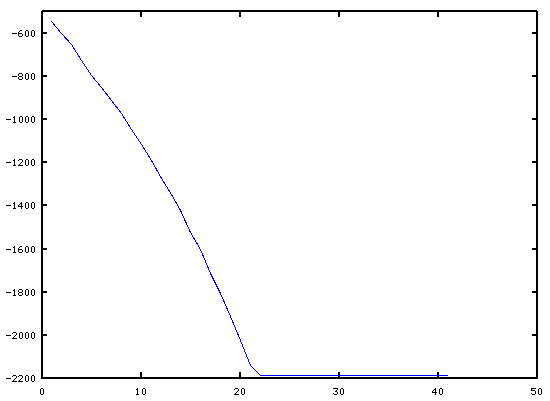
\includegraphics[scale=0.25]{../../src/img/results/energy_noise_50.png}}
 \caption{Energía en la evaluación de la entrada presentada.}
 \label{Fig:energy}
\end{figure}
\end{block}
\end{frame}

\begin{frame}{Mejor combinación}
%\begin{block}{Mejor combinación}
\begin{figure}[h!]
 \centering
 \fbox{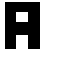
\includegraphics{../../src/img/original/a.png}}
 \fbox{
\includegraphics{../../src/img/original/bad-egg.png}}
 \fbox{
\includegraphics[scale=1.34]{../../src/img/original/circle-union.png}}
 \fbox{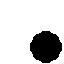
\includegraphics[scale=1.34]{../../src/img/original/circle1.png}}
 \fbox{
\includegraphics[scale=1.34]{../../src/img/original/footprint.png}}
 \fbox{
\includegraphics{../../src/img/original/line1.png}}
 \fbox{
\includegraphics{../../src/img/original/midnight-bsd.png}}
 \caption{Conjunto de patrones estables más grande.}
 \label{Fig:bestCombination}
\end{figure}
%\end{block}}
\end{frame}

\begin{frame}{Conclusiones}
\begin{block}{Conclusiones}
\begin{itemize}
\item Pudo notarse que además de existir los atractores correspondientes a los patrones almacenados en la red, existen otros atractores
 correspondientes a estados espurios.\\
 \item Los estados espurios correspondientes a los patrones almacenados invertidos poseen cuencas de atracción muy grandes
 y comparables con las de los patrones originales. 
 \item Los estados espurios conformados por la mezcla de patrones almacenados poseen una cuenca de atracción pequeña.\\
 \item Se pudo notar que al eliminar estados espurios de la red se puede afectar también a los patrones almacenados. 
 
\end{itemize}
\end{block}
\end{frame}
\end{document}
